\section{Effective Emails and Reports}

% TODO (maybe) https://graphthinking.blogspot.com/2020/09/identifying-and-eliminating.html

A common misconception is that emails and reports are for communication. To be more precise, the only true statement you can surmise from the activity is, ``I wrote something." 
Asynchronous communication has no requirement for a response or action. There's no guarantee that what you wrote has been incorporated into the audience's mental conception of reality. That's what makes it asynchronous. Any communication (i.e., building a shared mental model) that occurs is merely incidental.

Even though emails and reports may not be ideal forms of communication, there are other reasons they are useful to invest time in.

\ \\
\textit{Written documents as notifications}: Email can be used to document that you told someone something. Even if they don't read the content, you can later point out that the information was provided.

\ \\
\textit{Email as a task request}: Putting a task in another person's shifts the responsibility. Emails in their queue may or may not be read, and may or may not be acted upon. 

\ \\
Just because you sent an email or filed a report, your responsibility to communicate effectively hasn't finished. You need to confirm that the audience has integrated the information. 

\ \\
%***************************

%\subsection*{Email: A Piece of Art, A Form, and A Game\label{sec:art-form-game}}

Another reframing of emails and reports is to discard the concept of an essay. When you learned to write in school, you were taught the essay structure and associated conventions. Emails are not essays, and they don't have to conform to the norms of essays. Three ways of novel ways of thinking of emails are as a template, as art, and as a game.

\ \\
\textbf{Email is Structured}: Originality is not a requirement in bureaucratic writing. Plagiarism is acceptable. The consistency of a fill-in-the-blank 
%\href{https://en.wikipedia.org/wiki/Mad_Libs}{Mad Libs} 
%\index{Wikipedia!\href{https://en.wikipedia.org/wiki/Mad_Libs}{Mad Libs}}\iftoggle{WPinmargin}{\marginpar{$>$Wikipedia: Mad Libs}}{}
template for reports is efficient.  

\ \\
\textbf{Email is a Piece of Art}: Effort invested in each email to improve readability means more than just careful wording. 
Use visual cues (different fonts, different font sizes, highlighting, font color) and pictures to improve readability. See figure~\ref{fig:email_computer_font} for an example.

\ \\
\textbf{Email is a Game}: Email is a game of documenting decisions and responses so that the sequence of interactions is clear for audits and recrimination. 

\ \\
Your emails are not constrained to an essay-like narrative structure. 

\subsection*{Asynchronous Communication Responsiveness\label{sec:email-responsiveness}}

Delayed response applies to any asynchronous communication such as voicemail, email, memos,  and reports. Here I'll use email, though the same issues apply to other channels.


There are tiers of responsiveness, assuming the reader wants to respond but doesn't have sufficient time available.
(The explanations below can be the other side of \gls{stonewalling} or \gls{slow-rolling}.)
\iftoggle{glossaryinmargin}{\marginpar{[Glossary]}}{}

Which level you are at depends on the speed of your reading, how fast you can write, the number of incoming emails, the number of outgoing emails, and how much time you allocate for email. 
\begin{enumerate}
    \item You can read all incoming emails and reply to all emails that necessitate a response.
    \item You can read all emails and reply to some. 
    \begin{itemize}
        \item Only important emails.
        \item Only emails that have short answers.
    \end{itemize}
    \item You are unable to read all incoming emails. 
    \begin{itemize}
        \item Skim the content of all emails to find relevant information, but likely to miss some key points.
        \item Read emails from important people only (based on who the sender is).
        \item Search through your inbox if someone needs something and cites an email that was sent to you.
    \end{itemize}
    \item You have an assistant to respond to emails.
    \item You have a front office team to handle messaging.
\end{enumerate}
The following scenarios are focused on case 2, where you can triage (skim) emails but do not have enough time to respond to each.


In a situation where you have insufficient time, which of the following emails do you reply to? An email from your boss, an email from your peer, an email from a person who reports to you, or a person who you do not know?
(The ratio of these email categories is not one to one to one to one.)

The email from your boss is likely the top priority. Of the remaining emails (peer, subordinate, unknown), the peer email is likely the next priority.
The subordinate and unknown person are likely last.

The consequence of triage is that when there's insufficient time available, your transparency to subordinates and unknown people is likely to decrease. 

\ \\
Let's consider another scenario requiring triage of email. Three emails come in. One has no action, one is easy to reply to, and the third is difficult and takes time. Which one gets the response?
As with the previous scenario, the ratio of these inbound emails is not one to one to one.

The email that is easy to reply to gets answered first.  The difficult email is second.
If you only have time for one of the emails, it's likely to be the easy one. This is an example of 
\href{https://en.wikipedia.org/wiki/Ambiguity_aversion}{ambiguity aversion} -- preferring known over the unknown.
\index{Wikipedia!ambiguity aversion@\href{https://en.wikipedia.org/wiki/Ambiguity_aversion}{ambiguity aversion}}\iftoggle{WPinmargin}{\marginpar{$>$Wikipedia: Ambiguity\\aversion}}{}
As a consequence, outsiders see this as you demonstrating bikeshedding, also known as the
\href{https://en.wikipedia.org/wiki/Law_of_triviality}{Law of triviality}: disproportionate weight is given to trivial issues.
\index{Wikipedia!Law of triviality@\href{https://en.wikipedia.org/wiki/Law_of_triviality}{Law of triviality}}
\index{folk wisdom!Law of triviality@\href{https://en.wikipedia.org/wiki/Law_of_triviality}{Law of Triviality}}



\subsection*{Improving your Emails\label{sec:email-structure}}

\index{list of tips!email}

Whether you are the only recipient or one of many receivers can change the intent of the email. Whether you are in the ``to" or ``cc" field matters. Unfortunately, ``to" versus ``cc" are not reliable indicators since email senders do not reliably conform to the expected use. 


%This categorization of text within emails is a useful natural language processing challenge for machine learning. Currently a few email providers already do some of this with identifying meeting logistics, providing reminders to follow-up, and providing reply snippets. A browser plug-in that differentiates the various purposes of text could help readers determine relevant actions and responses. 

An email sent to multiple recipients may have different purposes for different readers. The reader's role or knowledge may factor into how they interpret the content. The inclusion or exclusion of recipients alters how the content is understood. 

\ \\
\textit{Email Improvement}: Good emails balance enough context (the why) and relevant details (the what) against conciseness (word count). 

\ \\
\textit{Email Improvement}: Emails convey both emotional tone and facts. Your intent as an author is practically irrelevant; the reader's perception is paramount. 


% from https://graphthinking.blogspot.com/2021/10/structuring-email-content-for.html

\ \\
\textit{Email Improvement}: Use consistent design and structure for your emails. Emails are part of your professional reputation. See Figure~\ref{fig:email_template}.

\ \\
\textit{Email Improvement}: Emails start with a greeting: Hi, Hello, Good morning, Good afternoon, Good evening. 
Email greetings include the name of the targeted recipient(s). See Figure~\ref{fig:email_two_questions}.

\ \\
\textit{Email Improvement}: Emails end with a professional closing, e.g., ``Kindly", ``Regards", etc. See Figure~\ref{fig:email_template}. % template

\ \\
\textit{Email Improvement}: Emails have a signature block with contact information -- phone number, normal hours of response, which timezone you're in if your team spans timezones, how long to wait for a response before asking again, which communication channel you prefer, etc. See Figure~\ref{fig:email_template}. % template

% https://www.overleaf.com/learn/latex/Errors/%60!h%27_float_specifier_changed_to_%60!ht%27
\begin{figure}%[H] % formerly ht
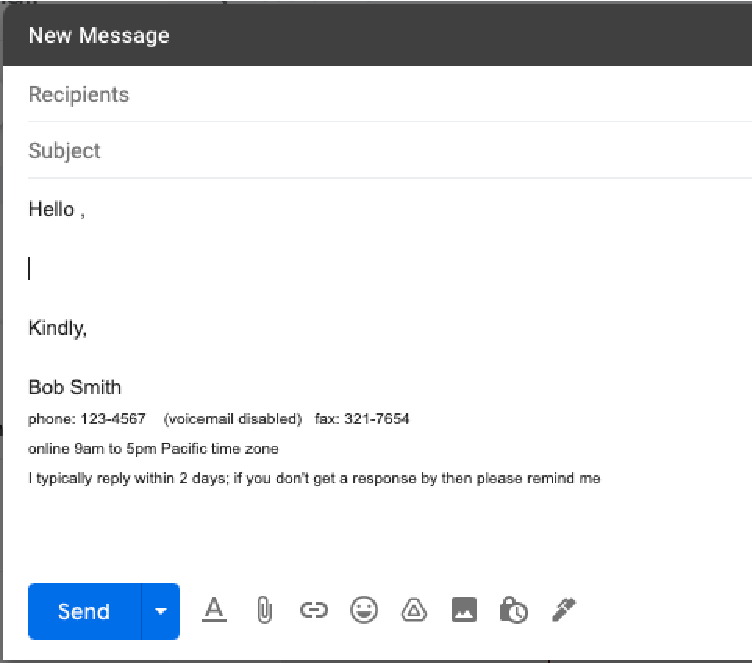
\includegraphics[width=1\textwidth]{images/email_template.pdf}
\caption{Template for new email messages. The greeting has a space after the comma -- that is where the recipient's name will go. Signature block uses a smaller font size after the name.}
\label{fig:email_template}
\end{figure}

\ \\
\begin{samepage}
\textit{Email Improvement}: Email signature blocks do not include unnecessary images, as that uses more storage for recipients.
\end{samepage}

\ \\
\begin{samepage}
\textit{Email Improvement}: Email threads focused on a specific instance of a recurring event include the date (YYYY-MM-DD) in the subject line. See Figure~\ref{fig:email_meeting_notes}.
\end{samepage}

\ \\
\begin{samepage}
\textit{Email Improvement}: Based on the purpose of the email, example key phrases for subject lines include: ``meeting notes" versus ``agenda" versus ``question about."
\end{samepage}

\ \\
\begin{samepage}
\textit{Email Improvement}: Revising an existing subject line can disrupt the ability of email software to thread conversations. However, sometimes the revision is worth breaking threading.
\end{samepage}

\ \\
\begin{samepage}
\textit{Email Improvement}: When replying to an ongoing thread, keep the original message as part of the thread to provide readers with historical context.
\end{samepage}

\ \\
\begin{samepage}
\textit{Email Improvement}: When replying to threads with sensitive messages, sanitize the included content by removing names or identifying details.
\end{samepage}

\ \\
\begin{samepage}
\textit{Email Improvement}: If an email has multiple requests or questions, at the top of the email (after the greeting) explicitly say how many of each type. Then, in the body of the message, number them. See Figure~\ref{fig:email_meeting_notes}.
\end{samepage}

% https://www.overleaf.com/learn/latex/Errors/%60!h%27_float_specifier_changed_to_%60!ht%27
\begin{figure}%[H] % formerly ht
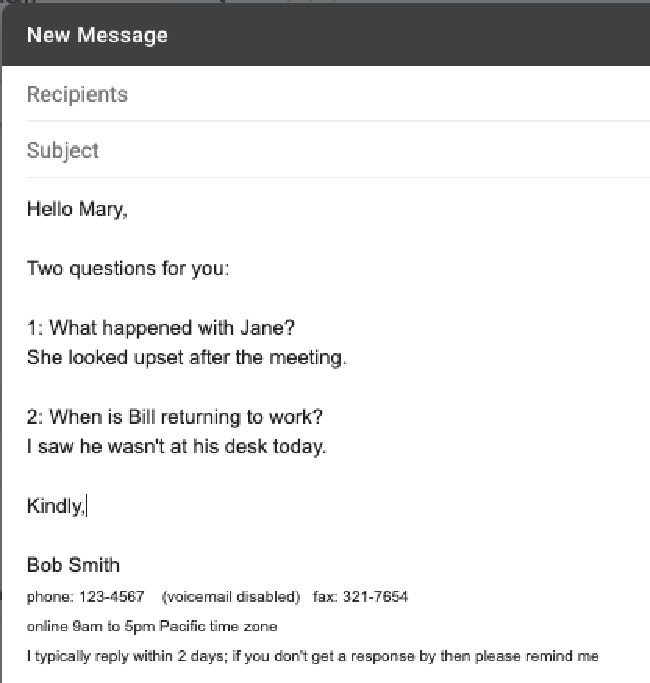
\includegraphics[width=1\textwidth]{images/email_two_questions.pdf}
\caption{Distinct items the recipient should address in a reply. A good subject for this email would indicate there are two questions you are seeking answers for.}
\label{fig:email_two_questions}
\end{figure}

\ \\
\begin{samepage}
\textit{Email Improvement}: If an item corresponds to a requested action, separately highlight the action and indicate who is supposed to take the action and what the deadline for response is.
\end{samepage}

% https://www.overleaf.com/learn/latex/Errors/%60!h%27_float_specifier_changed_to_%60!ht%27
\begin{figure}%[H] % formerly ht
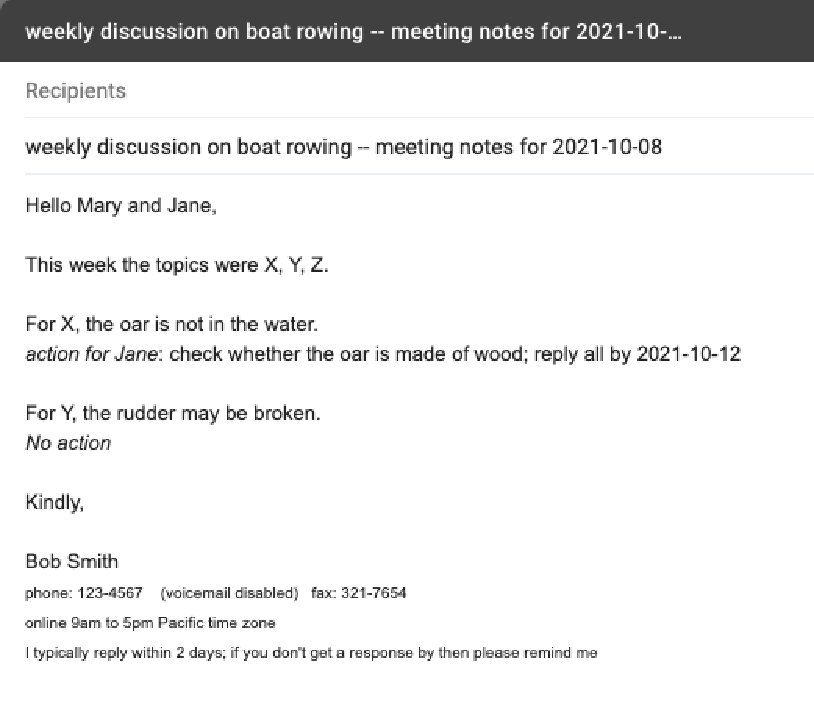
\includegraphics[width=1\textwidth]{images/email_meeting_notes.pdf}
\caption{Who has what action due when? The meeting notes are for a particular instance of a recurring event, so YYYY-MM-DD is included in the subject. Process Empathy involves thinking ahead about how future readers will differentiate this message from others.}
\label{fig:email_meeting_notes}
\end{figure}

\ \\
\begin{samepage}
\textit{Email Improvement}: Computer commands should use distinct separate fixed-width font. This distinguishes the text from the rest of the narrative.  See Figure~\ref{fig:email_computer_font}.
\end{samepage}


\begin{figure}%[H] % formerly ht
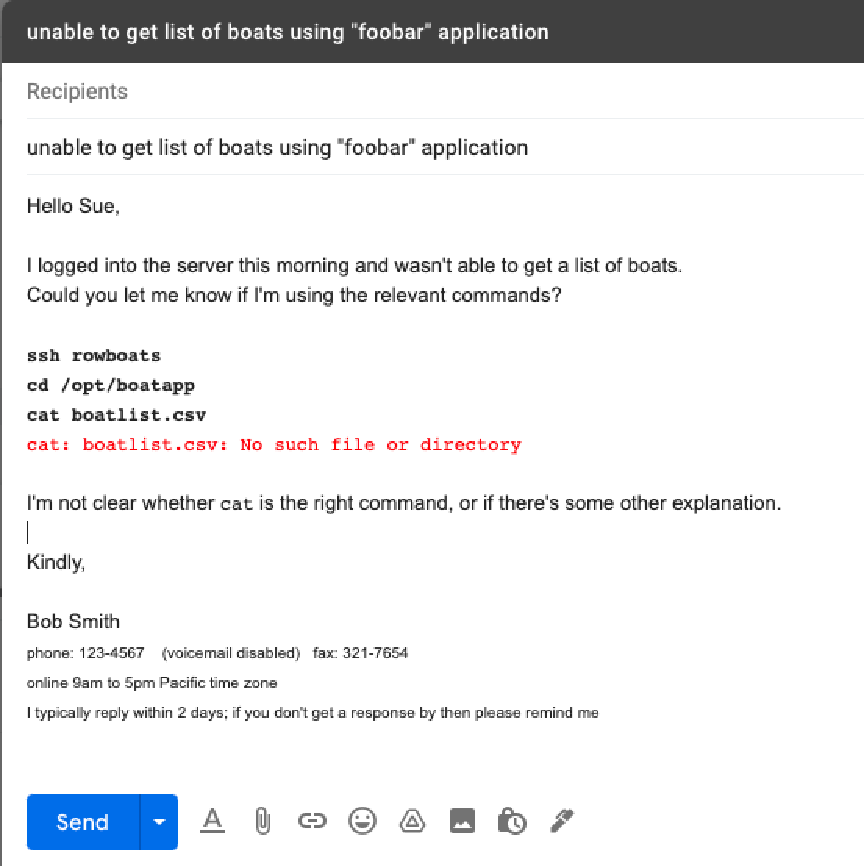
\includegraphics[width=1\textwidth]{images/email_computer_font.pdf}
\caption{The computer commands use fixed-width font. Input is distinguished from output using of bold and non-bold respectively. The error message is highlighted using red. Inline text like ``cat'' in the last line is also fixed width.}
\label{fig:email_computer_font}
\end{figure}

\ \\
\begin{samepage}
\textit{Email Improvement}: References to documents include a direct full path.
\end{samepage}

\ \\
\begin{samepage}
\textit{Email Improvement}: If referring to a previous separate thread, include the subject and the date+time that email was sent.
\end{samepage}

\ \\
\begin{samepage}
\textit{Email Improvement}: For bullet points, explicitly specify that items are joined by one of the following: OR, XOR, AND. For example,
\begin{itemize}
    \item Buy bread.\\
    \textit{and}
    \item Sell socks.
\end{itemize}
versus
\begin{itemize}
    \item Press the ``Return'' key.\\
    \textit{xor}
    \item Press the ``Space'' key.
\end{itemize}
\end{samepage}

\ \\
\begin{samepage}
\textit{Email Improvement}: If you have an unordered list, explicitly state that order is irrelevant.
\end{samepage}

\ \\
\begin{samepage}
\textit{Email Improvement}: If you have a sequence of steps, number them and indicate which steps are required versus optional. For example,
\begin{enumerate}
    \item (\textit{required}) Go to France.
    \item (\textit{optional}) Go to Greece.
    \item (\textit{required}) Go to Spain.
\end{enumerate}
\end{samepage}

\ \\
\begin{samepage}
\textit{Email Improvement}: Use visual sketches to illustrate concepts rather than always relying on text. Don't use pictures all the time, and don't have too many pictures in an email. 
\end{samepage}

\ \\
\begin{samepage}
\textit{Email Improvement}: Know how to both embed pictures inline and how to attach files and when to use which. 
Email replies should preferentially be at the top of the thread. 
If replying to multiple points in the previous email, embed replies inline, mark the distinction, and highlight the authorship. 
\end{samepage}

\begin{figure}[H] % formerly ht
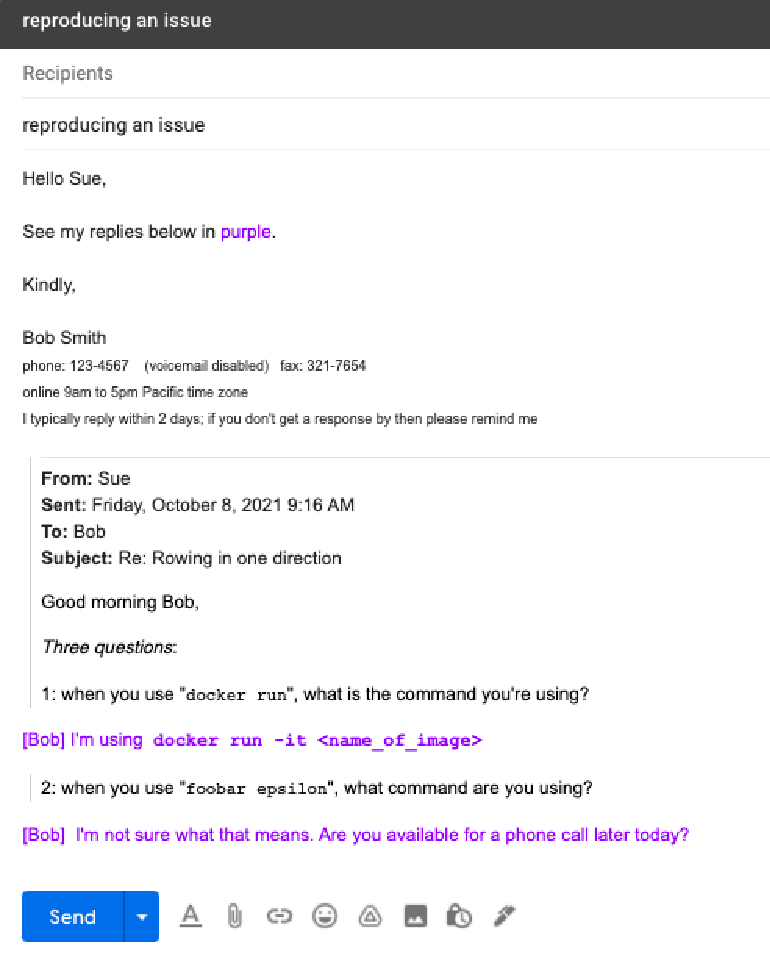
\includegraphics[width=1\textwidth]{images/email_reply.pdf}
\caption{Bob's reply to Sue's questions. The third question is not shown in this illustration.}
\label{fig:email_reply}
\end{figure}

\ \\
\begin{samepage}
\textit{Email Improvement}: If replying inline, explicitly state that at the top of the thread.
\end{samepage}

\ \\
\begin{samepage}
\textit{Email Improvement}: If the email is longer than a paragraph, provide a \href{https://en.wikipedia.org/wiki/BLUF_(communication)}{B.L.U.F}  (bottom line up front)
\index{Wikipedia!BLUF@\href{https://en.wikipedia.org/wiki/BLUF_(communication)}{BLUF}}\iftoggle{WPinmargin}{\marginpar{$>$Wikipedia: BLUF}}{}
or 
\href{https://en.wikipedia.org/wiki/TL;DR}{tl;dr} (too long; didn't read)
\index{Wikipedia!tl;dr@\href{https://en.wikipedia.org/wiki/TL;DR}{tl;dr}}
or summary. In general emails should be short. Longer discussions should be held on the phone or in person, with a summary report after the discussion. Reliance on a BLUF or tl;dr risks resulting in the reader skipping the content. 
\end{samepage}

\ \\
\begin{samepage}
\textit{Email Improvement}: Every email should have a purpose. What are you asking the recipient to do? How do you want them to feel? How should they respond?
\end{samepage}

\ \\
\begin{samepage}
\textit{Email Improvement}: When replying, starting your email with an expression of gratitude for the work the recipient has done so far sets a positive tone by acknowledging their investment.
\end{samepage}

\ \\
\begin{samepage}
\textit{Email Improvement}: Read each email and report to determine the purpose. 
\end{samepage}

Reading each email is burdensome. If you don't have time to read everything, a common tactic is to skim the content. 
% https://graphthinking.blogspot.com/2021/03/read-each-email-to-determine-purpose.html
This tactic of skimming can lead to problematic behavior. First you scan the text of a message to see if there is immediate action or response needed. If no action or response is needed, go to the next email. 
That may not work for emails that have logistics associated with future events, or emails that alter your perception of the situation.

If you read an email to figure out the purpose of the email, that will help determine what action and response are relevant. Here I'm using ``action" to refer to activities outside the email channel. 


\subsection*{Why did this Email get sent?}
Below are potential intentions of the person writing the email. 

\ \\
\begin{samepage}
\textit{Email intent}: \textbf{Decision needed}. Typically includes context. \\
\textit{Action}: if the team maintains a decision log, update that.
Response is your selection of a choice.
\end{samepage}

\textit{Improvement for decision-centric emails}: Instead of asking for a decision, ask if the person is opposed. Or, even better, ask for the go-ahead. 
This framing biases the respondent towards action (specifically approval) rather than thinking. 
See 
\hyperref[sec:approval-forgiveness-opposition]{approval and forgiveness and opposition}
\marginpar{See page~\pageref{sec:approval-forgiveness-opposition}.}
for more details.

\ \\
\begin{samepage}
\textit{Email intent}: \textbf{Situational awareness}.\\
\textit{Action}: Expected default is no action, but interject if there's an issue.
\end{samepage}

\ \\
\begin{samepage}
\textit{Email intent}: \textbf{Action or Tasking}.\\
\textit{Action}: Do something within a specified deadline.
\end{samepage}

\ \\
\begin{samepage}
\textit{Email intent}: \textbf{Approval sought}.\\
\textit{Action}: Confirm or deny.
\end{samepage}

\ \\
\begin{samepage}
\textit{Email intent}: \textbf{Feedback sought}.\\
\textit{Action}: Assessment of proposal.
\end{samepage}

\ \\
\begin{samepage}
\textit{Email intent}: \textbf{Meeting logistics}. Can be an announcement (widely available), registration (limited attendance), or invitation (specific to you). Attendance is either optional or required. \\
\textit{Action}: Create or update a calendar event.
Response should restate the logistics (specifically the time and date and location and purpose) to confirm. 
\end{samepage}

\ \\
\begin{samepage}
\textit{Email intent}: \textbf{Brainstorming}.\\
May provoke a response for building on an idea.
``For your situational awareness, no action needed." Notification of activity by someone else. Or change in plans. 
If needed, a correction to the described direction might trigger a response or even a meeting.
\end{samepage}

\ \\
\begin{samepage}
\textit{Email intent}: \textbf{Reference}. E.g., describing a process, or a business workflow, or a citation.\\
\textit{Action}: Copy process documentation to wiki. Copy citation to bibliography.
Acknowledgement response thanking the sender for the update or clarification.
\end{samepage}

\ \\
\begin{samepage}
\textit{Email intent}: \textbf{Setting a formal policy or issuing an informal edict}.\\
\textit{Action}: move the policy or edict documentation to \href{https://en.wikipedia.org/wiki/Confluence_(software)}{Confluence}
\index{Wikipedia!Confluence software@\href{https://en.wikipedia.org/wiki/Confluence_(software)}{Confluence}}
or Wiki.\iftoggle{WPinmargin}{\marginpar{$>$Wikipedia: Confluence}}{}
Acknowledgement response needed only if the edit is aimed at just me or the group I am leading.
\end{samepage}

\ \\
\begin{samepage}
\textit{Email intent}: \textbf{Question}.\\
If this is a recurring question, move to a ``Frequently Asked Questions" page on a Confluence or Wiki.
Response is needed that provides an answer or seeks clarification.
\end{samepage}

\ \\

By categorizing the intent of emails and reports, you can respond more appropriately. Often the intent may be unclear, in which case a response can be framed as curiosity-based: ``I think you're seeking a decision, but here's the question that is crucial to ask before deciding."

\ \\

% TRANSITION to 